\chapter{Định lý Liouville và dòng Hamilton}

\lectureoverview{Các phương trình Hamilton không chỉ đơn thuần viết lại các phương trình chuyển động dưới một dạng khác. Chúng xác định một trường vận tốc trên không gian pha mà độ phân kỳ bằng không. Sự triệt tiêu đơn giản đó chính là định lý Liouville: sự tiến hóa Hamilton bảo toàn thể tích trong không gian pha. Chúng ta sẽ đi tới định lý này theo đúng trình tự mà ý nghĩa của nó dần hiện rõ---trước hết là bảo toàn năng lượng, rồi đến các mặt năng lượng không đổi, tiếp theo là một chất lưu gồm các điều kiện đầu khả dĩ, và cuối cùng là sự tương phản giữa dòng chảy bảo toàn thể tích và một điểm hút tiêu tán. Chính ngôn ngữ ấy cũng dẫn một cách tự nhiên đến ngoặc Poisson.}

\section{Vì sao cần một dạng khác của cơ học?}

Định lý ta cần là đối ứng cổ điển liên tục của các sơ đồ trạng thái thuận nghịch được giới thiệu ở đầu môn học. Trong một quy luật rời rạc thuận nghịch, mỗi trạng thái có một mũi tên đi vào và một mũi tên đi ra. Hiện tại đủ để xác định cả trạng thái kế tiếp lẫn trạng thái ngay trước đó. Một quy luật tồi dồn nhiều trạng thái vào cùng một hố hút: tương lai có thể được xác định, nhưng quá khứ thì không còn khôi phục được.

Định lý Liouville nói điều gì xảy ra với sự phân biệt ấy khi tập trạng thái là một không gian pha liên tục. Cụm từ thay cho một mũi tên đi vào và một mũi tên đi ra sẽ là \emph{lưu lượng đi vào bằng lưu lượng đi ra}. Tuy nhiên, trước khi có thể diễn đạt cụm đó bằng toán học, ta cần dựng lại dòng từ các phương trình Hamilton.

Có một điều gây băn khoăn về mặt lịch sử khi làm việc này. Hamilton, Jacobi, Lagrange và Poisson đã xây dựng những hình thức cơ học cổ điển công phu và đẹp đẽ mà không hề biết đến lý thuyết lượng tử, nơi các hình thức đó sẽ trở nên không thể thiếu. Newton có một mục tiêu trực tiếp: chuyển động hành tinh. Lagrange và Hamilton cũng có trước mắt các bài toán vật lý, nhưng họ theo đuổi những phép tương tự và những cấu trúc vượt xa bất kỳ một quỹ đạo riêng lẻ nào. Nguyên lý tác dụng dừng trong cơ học giống với các nguyên lý thời gian cực tiểu trong quang học; chuyển động của tia và chuyển động của hạt có thể được đặt vào những dạng toán học song song. Họ đơn giản hóa, sắp xếp lại và thống nhất các phương trình vì bản thân các cấu trúc ấy dường như đã chứa đựng vật lý.

Giờ đây ta biết rằng trực giác ấy cực kỳ hiệu quả. Về mặt lôgic, nhiều đặc trưng của cơ học cổ điển có thể được hiểu như các giới hạn của cơ học lượng tử. Về mặt lịch sử, thứ tự lại đảo ngược: các cấu trúc cổ điển được tìm ra trước, và chỉ mãi về sau công dụng sâu hơn của chúng mới trở nên rõ ràng. Một câu đùa khiêu khích thường được gán cho Feynman đã nêu bật điểm này bằng cách đối lập toán học được theo đuổi từ bên trong với vật lý bị ràng buộc bởi một đối tác bên ngoài, là thế giới vật lý. Câu đùa không phải là một lập luận, nhưng sự phân biệt ấy là hữu ích: vẻ đẹp hình thức có ý nghĩa ở đây vì tự nhiên nhiều lần lựa chọn chính các cấu trúc hình thức này.

\begin{classroomqa}\audiencequestion{Newton đã có khái niệm hiện đại về động năng chưa, và khái niệm năng lượng bắt đầu từ đâu?\lecturetimestamp{00:04:24--00:05:50}}\lecturerresponse{Cơ học của Newton được tổ chức quanh lực và chuyển động, chứ không quanh một nguyên lý năng lượng tổng quát đã chín muồi. Vấn đề ai có trước một cách chính xác về mặt lịch sử không được phân định dứt khoát trong phần thảo luận này. \emph{vis viva} của Leibniz, \(\sum_i m_i v_i^2\), là một tiền thân quan trọng và bằng hai lần động năng hiện đại. Công trình về nhiệt về sau đã khiến sự chuyển đổi giữa nhiệt và công cơ học trở thành trung tâm. Các lý thuyết nhiệt tố ban đầu xem nhiệt như một chất được bảo toàn, vì vậy ý niệm hiện đại về các dạng năng lượng có thể chuyển hóa lẫn nhau chỉ xuất hiện dần dần.}\end{classroomqa}

\section{Các phương trình Hamilton và bảo toàn năng lượng}

Xét một hệ có \(n\) cặp chính tắc, \begin{equation}
  (q_i,p_i),\qquad i=1,\ldots,n.
  \label{eq:l7-canonical-pairs}
\end{equation} Mỗi tọa độ đi kèm một động lượng và mỗi động lượng đi kèm một tọa độ. Quy luật chuyển động được gói gọn trong một hàm, \begin{equation}
  H=H(q_1,\ldots,q_n,p_1,\ldots,p_n,t),
  \label{eq:l7-hamiltonian}
\end{equation} và các phương trình Hamilton là \begin{equation}
  \boxed{
  \dot q_i=\frac{\partial H}{\partial p_i},
  \qquad
  \dot p_i=-\frac{\partial H}{\partial q_i}.}
  \label{eq:l7-hamilton-equations}
\end{equation} Dấu là một phần của cấu trúc chính tắc. Phương trình \(q\) mang dấu cộng; phương trình \(p\) mang dấu trừ.

\begin{figure}[htbp]\centering
  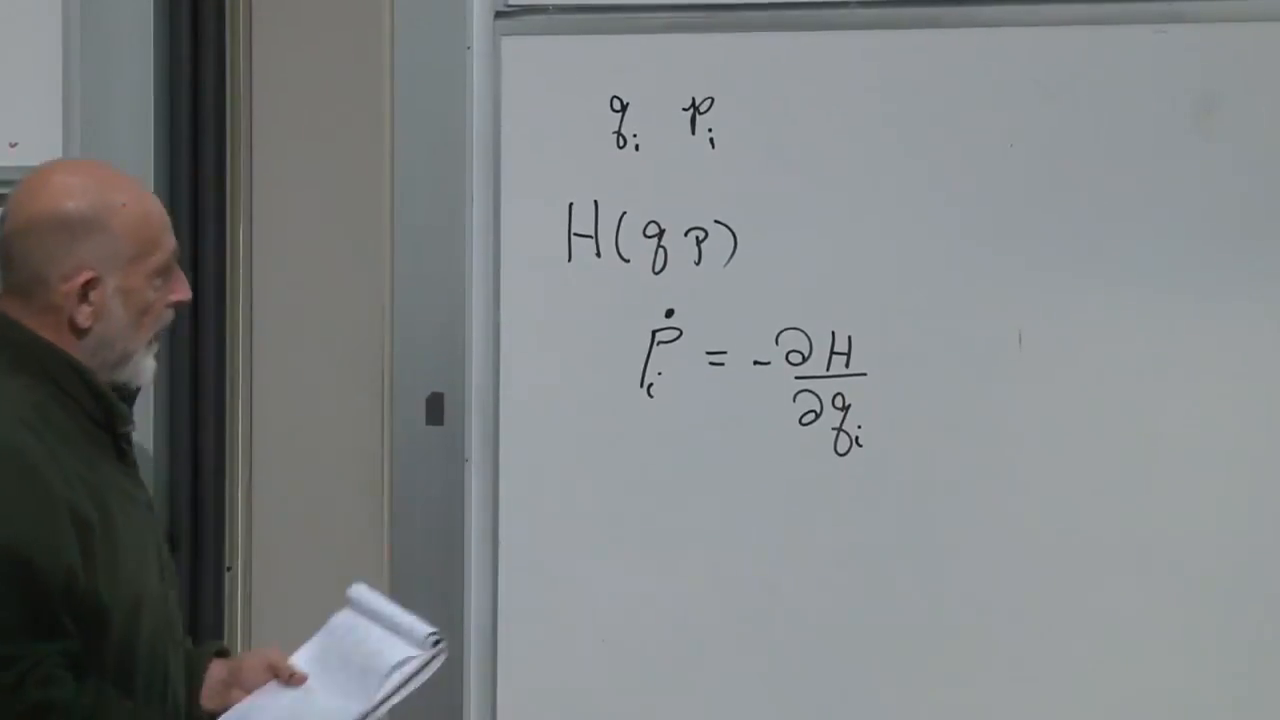
\includegraphics[width=0.82\textwidth]{lecture_07_figure_02.png}\caption{Các biến chính tắc, hàm \(H(q,p)\) và phương trình Hamilton phía động lượng ở phần đầu của phần điểm lại.}\lectureframe{00:07:29}\end{figure}

Mặc dù các phương trình được viết thành những cặp có chỉ số, động lực học không nhất thiết tách riêng thành từng cặp. Hamiltonian có thể ghép mọi \(q_i\) và \(p_i\) với nhau, nên chẳng hạn \(\dot p_1\) có thể phụ thuộc vào trạng thái của toàn bộ hệ.

\begin{classroomqa}\audiencequestion{Cách trình bày đến đây có phải là mang tính tiên đề không? Ta đã giả sử quan hệ nào giữa \(p\) và \(q\)?\lecturetimestamp{00:17:08--00:18:18}}\lecturerresponse{Các phương trình Hamilton xác định lý thuyết hình thức một khi \(H(q,p)\) và các cặp chính tắc đã được chỉ ra. Không có giả thiết bổ sung phổ quát nào rằng \(p=m\dot q\). Quan hệ ấy đúng với một hạt thông thường trong hệ tọa độ Descartes với động năng bậc hai, nhưng các tọa độ khác và các Hamiltonian khác cho những quan hệ động lượng--vận tốc khác. Bản thân các phương trình cung cấp quan hệ đó thông qua \(\dot q_i=\partial H/\partial p_i\). Việc một Hamiltonian được đề xuất có được hiện thực hóa trong tự nhiên hay không lại là một câu hỏi vật lý khác.}\end{classroomqa}

Giờ ta có thể thu lại sự bảo toàn năng lượng bằng một mạch suy luận. Dọc theo một quỹ đạo, đạo hàm toàn phần của \(H\) là \begin{equation}
  \frac{dH}{dt}
  =
  \sum_i\left(
    \frac{\partial H}{\partial q_i}\dot q_i
    +\frac{\partial H}{\partial p_i}\dot p_i
  \right)
  +\frac{\partial H}{\partial t}.
  \label{eq:l7-total-h-derivative}
\end{equation} Hạng cuối cùng biểu thị sự phụ thuộc tường minh vào thời gian khi giữ cố định \(q\) và \(p\), có thể là vì một tham số do bên ngoài ấn định đang thay đổi. Thay phương trình~\eqref{eq:l7-hamilton-equations} vào, \begin{align}
  \frac{dH}{dt}
  &=
  \sum_i\left[
    \frac{\partial H}{\partial q_i}
    \frac{\partial H}{\partial p_i}
    -\frac{\partial H}{\partial p_i}
    \frac{\partial H}{\partial q_i}
  \right]
  +\frac{\partial H}{\partial t}\\
  &=\frac{\partial H}{\partial t}.
  \label{eq:l7-h-energy-rate}
\end{align} Mỗi hạng trong tổng triệt tiêu với hạng đối ứng của nó. Do đó, \begin{equation}
  \frac{\partial H}{\partial t}=0
  \quad\Longrightarrow\quad
  \frac{dH}{dt}=0.
  \label{eq:l7-energy-conservation}
\end{equation} Đối với một hệ kín bất biến theo tịnh tiến thời gian, Hamiltonian được bảo toàn và chính là năng lượng.

\begin{classroomqa}\audiencequestion{Điều gì thay đổi nếu Hamiltonian phụ thuộc tường minh vào thời gian? \lecturetimestamp{00:10:32--00:12:33}}\lecturerresponse{Khi đó phương trình~\eqref{eq:l7-h-energy-rate} vẫn đúng, nhưng năng lượng của hệ con không nhất thiết không đổi. Sự phụ thuộc tường minh vào thời gian thường biểu diễn một tác nhân dẫn động bị lược bỏ đang trao đổi năng lượng với hệ. Nếu tác nhân ấy được nâng lên thành một phần động lực học của một hệ kín lớn hơn, Hamiltonian của hệ lớn hơn lại có thể không phụ thuộc thời gian và tổng năng lượng của nó được bảo toàn.}\end{classroomqa}

\section{Năng lượng như hình học trong không gian pha}

Bây giờ giả sử \(H\) không phụ thuộc tường minh vào thời gian. Điều kiện đầu xác định một giá trị \(E\), và điểm pha vẫn nằm trên \begin{equation}
  H(q,p)=E.
  \label{eq:l7-energy-surface}
\end{equation} Không gian pha có \(2n\) chiều. Tại các điểm chính quy, một phương trình theo các tọa độ của nó xác định một siêu mặt \((2n-1)\) chiều. Những giá trị khác nhau của \(E\) cho những siêu mặt khác nhau. Chúng không nhất thiết kín hay compact; bảo toàn năng lượng chỉ nói rằng một quỹ đạo bắt đầu trên một trong các siêu mặt ấy sẽ không bao giờ rời khỏi nó.

Đối với dao động tử điều hòa đã hiệu chỉnh ở bài giảng trước, \begin{equation}
  H=\frac{\omega}{2}(p^2+q^2).
  \label{eq:l7-oscillator-hamiltonian}
\end{equation} Vì thế mỗi tập năng lượng không đổi là một đường tròn, \begin{equation}
  p^2+q^2=\frac{2E}{\omega}.
  \label{eq:l7-oscillator-circle}
\end{equation}

\begin{figure}[htbp]\centering
  \includegraphics[width=0.84\textwidth]{lecture_07_figure_04.png}\caption{Phác họa không gian pha \(2n\) chiều và Hamiltonian của dao động tử điều hòa dùng để giới thiệu các mặt năng lượng không đổi.}\lectureframe{00:15:20}\end{figure}

Các phương trình chuyển động, \begin{equation}
  \dot q=\omega p,\qquad \dot p=-\omega q,
  \label{eq:l7-oscillator-flow}
\end{equation} làm cho điểm ấy chuyển động theo chiều kim đồng hồ quanh đường tròn của nó. Phương trình năng lượng cho ta biết chuyển động nằm trên đường cong nào; các phương trình Hamilton cho ta biết hướng và tốc độ dọc theo đường cong đó.

\begin{figure}[htbp]\centering
  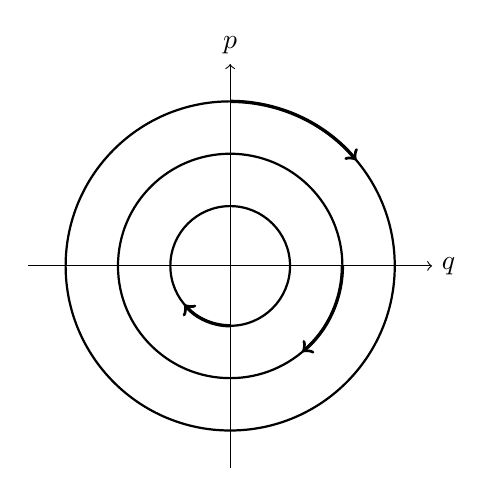
\begin{tikzpicture}[scale=0.95]
    \draw[->] (-2.7,0) -- (2.7,0) node[right] {\(q\)};
    \draw[->] (0,-2.7) -- (0,2.7) node[above] {\(p\)};
    \draw[thick] (0,0) circle (0.8);
    \draw[thick] (0,0) circle (1.5);
    \draw[thick] (0,0) circle (2.2);
    \draw[->,very thick] (0,2.2) arc[start angle=90,end angle=40,radius=2.2];
    \draw[->,very thick] (1.5,0) arc[start angle=0,end angle=-50,radius=1.5];
    \draw[->,very thick] (0,-0.8) arc[start angle=-90,end angle=-140,radius=0.8];
  \end{tikzpicture}\caption{Năng lượng không đổi cho các đường tròn; các phương trình dao động tử cho dòng tiếp tuyến theo chiều kim đồng hồ.}\end{figure}

\begin{classroomqa}\audiencequestion{Hai phương trình Hamilton và \(H=E\) có phải là nhiều phiên bản của cùng một phương trình không?\lecturetimestamp{00:15:53--00:17:06}}\lecturerresponse{Không. Các phương trình Hamilton là hai quy luật chuyển động bậc một cho một cặp chính tắc. Chúng kéo theo \(dH/dt=0\), từ đó suy ra \(H=E\). Giá trị của \(E\) được chọn bởi điều kiện đầu. Phương trình \(H=E\) xác định một mặt; tự nó không quy định vận tốc dọc theo mặt đó.}\end{classroomqa}

\section{Từ một trạng thái đến một dòng các trạng thái}

Thay vì theo dõi một điều kiện đầu, hãy rải khắp không gian pha mọi điều kiện đầu có thể có rồi cho đồng hồ chạy. Mỗi điểm là một trạng thái khả dĩ hoàn chỉnh, và mỗi trạng thái chuyển động theo các phương trình Hamilton. Có thể hình dung sự rải đó như một đám bụi hay một chất lưu tưởng tượng. Không có vật chất nào thực sự được đổ vào không gian pha; chất lưu chỉ là một cách để nhìn thấy mọi quỹ đạo cùng một lúc.

Trường vận tốc trong không gian pha là \begin{equation}
  \mathbf V(q,p,t)
  =
  (\dot q_1,\ldots,\dot q_n,\dot p_1,\ldots,\dot p_n).
  \label{eq:l7-phase-velocity}
\end{equation} Với một cặp chính tắc, ta viết \begin{equation}
  V_q=\dot q=\frac{\partial H}{\partial p},
  \qquad
  V_p=\dot p=-\frac{\partial H}{\partial q}.
  \label{eq:l7-phase-components}
\end{equation} Tại mỗi điểm, Hamiltonian gán một vectơ cho biết điểm pha sẽ đi đâu tiếp theo. Nếu \(H\) không phụ thuộc thời gian, trường vectơ là dừng: trở lại cùng một điểm pha sẽ cho cùng một vận tốc. Nếu \(H\) phụ thuộc vào thời gian, chính trường vectơ thay đổi theo thời gian, nhưng nó vẫn được xác định ở mỗi thời điểm.

\begin{figure}[htbp]\centering
  \includegraphics[width=0.84\textwidth]{lecture_07_figure_05.png}\caption{Trường vận tốc của dao động tử điều hòa. Các vectơ tiếp tuyến với các đường tròn và ngắn dần về phía gốc tọa độ.}\lectureframe{00:24:50}\end{figure}

Đối với dao động tử điều hòa, mọi bán kính đều quay với tốc độ góc \(\omega\). Các điểm gần gốc có tốc độ tuyến tính nhỏ hơn vì chúng đi trên một đường tròn ngắn hơn trong cùng một chu kỳ. Vì vậy toàn bộ đám bụi quay như một bàn quay cứng.

\begin{classroomqa}\audiencequestion{Sự quay cứng có nghĩa là mọi quỹ đạo của dao động tử đều có cùng chu kỳ phải không? \lecturetimestamp{00:21:10--00:21:42}}\lecturerresponse{Có. Tính không phụ thuộc vào biên độ ấy là tính chất đặc trưng xác định của dao động tử điều hòa. Mọi đường tròn đều được đi quanh với cùng tần số góc \(\omega\), mặc dù độ lớn của vận tốc trong không gian pha nhỏ hơn trên một đường tròn nhỏ hơn.}\end{classroomqa}

\begin{classroomqa}\audiencequestion{Vận tốc trong không gian pha có giống nhau tại mọi điểm không?\lecturetimestamp{00:24:29--00:25:37}}\lecturerresponse{Không. Cả hướng lẫn độ lớn của nó nói chung đều thay đổi theo vị trí. Với dao động tử, vectơ tiếp tuyến với đường tròn tại điểm đó và có độ lớn \(\omega\sqrt{p^2+q^2}\). Một trường vectơ nghĩa là ở mỗi điểm đều có một vectơ được gán vào, chứ không phải một vectơ giống hệt được sao chép khắp nơi.}\end{classroomqa}

\begin{classroomqa}\audiencequestion{Chính xác thì các hạt và mật độ của chất lưu tưởng tượng này là gì? \lecturetimestamp{00:56:03--00:58:40}}\lecturerresponse{Mỗi điểm là một trạng thái hoàn chỉnh của toàn bộ hệ cơ học. Nó không phải là một hạt vật lý. 5 hạt chuyển động trong một chiều không gian cần 5 vị trí và 5 động lượng, vì thế không gian pha có 10 chiều; trong 3 chiều thì cần 30 chiều. Đám bụi là một tập hợp các trạng thái thay thế. Nếu hình ảnh chất lưu gây xao lãng, chỉ cần lấy một miền điều kiện đầu, cho mọi điểm trong đó tiến hóa, rồi so sánh thể tích không gian pha của miền ấy trước và sau.}\end{classroomqa}

\section{Sự nén và độ phân kỳ}

Để hỏi xem chất lưu tưởng tượng này có mất thể tích hay không, trước hết xét một chiều. Cho các điểm trên một đường thẳng chuyển động với vận tốc \(v(x)\). Hai điểm gần nhau cách nhau \(\delta x\) có hiệu vận tốc \begin{equation}
  \delta v \simeq \frac{dv}{dx}\,\delta x.
  \label{eq:l7-one-dimensional-strain}
\end{equation} Nếu \(dv/dx>0\), điểm ở phía trước chuyển động nhanh hơn và khoảng cách dãn ra. Nếu \(dv/dx<0\), nó bị nén lại. Vì vậy, một dòng một chiều dừng và không nén được phải thỏa \begin{equation}
  \frac{dv}{dx}=0.
  \label{eq:l7-one-dimensional-incompressible}
\end{equation}

\begin{figure}[htbp]\centering
  \includegraphics[width=0.84\textwidth]{lecture_07_figure_06.png}\caption{Lập luận một chiều dẫn tới \(dv/dx\) như tốc độ dãn hoặc nén cục bộ.}\lectureframe{00:30:20}\end{figure}

Có hai cách nhìn tương đương. Ta có thể theo dõi một đoạn vật chất và hỏi xem độ dài của nó có thay đổi hay không. Hoặc ta có thể giữ cố định một đoạn nhỏ và hỏi xem lượng đi vào trong một đơn vị thời gian có bằng lượng đi ra hay không. Cách thứ nhất đi theo chất lưu; cách thứ hai quan sát nó đi qua.

Trong nhiều hơn một chiều, một miền có thể dãn theo một trục và nén theo một trục khác mà không làm thay đổi tổng thể tích. Đối với trường vận tốc \(\mathbf V=(V_x,V_y,V_z)\), tốc độ cục bộ thích hợp là độ phân kỳ, \begin{equation}
  \nabla\cdot\mathbf V
  =
  \frac{\partial V_x}{\partial x}
  +\frac{\partial V_y}{\partial y}
  +\frac{\partial V_z}{\partial z}.
  \label{eq:l7-spatial-divergence}
\end{equation} Độ phân kỳ dương là sự giãn nở cục bộ, độ phân kỳ âm là sự co lại cục bộ, và điều kiện không nén được là \begin{equation}
  \nabla\cdot\mathbf V=0.
  \label{eq:l7-zero-divergence}
\end{equation} Dòng vào và dòng ra bằng nhau qua một hộp nhỏ cố định là cùng một phát biểu cục bộ với việc bảo toàn thể tích của một hộp nhỏ chuyển động.

\begin{figure}[htbp]
  \centering
  \includegraphics[width=0.86\textwidth]{lecture_07_figure_07.png}
  \caption{Một ô hai chiều, các thành phần dòng của nó, và tổng các đạo hàm theo cùng tọa độ xác định độ phân kỳ.}
  \lectureframe{00:35:30}
\end{figure}

\begin{classroomqa}
  \audiencequestion{Chúng ta đang bàn về một chất lưu trong không gian thông thường hay một dòng trong không gian pha? \lecturetimestamp{00:34:27--00:34:40}}
  \lecturerresponse{Lập luận về độ phân kỳ trước hết là một lập luận tổng quát về chất lưu.
  Chúng ta sẽ áp dụng nó cho không gian pha có số chiều chẵn, trong đó các hướng tọa độ
  là \(q_i\) và \(p_i\), còn các thành phần vận tốc là
  \(\dot q_i\) và \(\dot p_i\).}
\end{classroomqa}

Giờ quay lại các ánh xạ trạng thái rời rạc. Trong một chu trình thuận nghịch, mỗi nút có
một mũi tên đi vào và một mũi tên đi ra, và một tập hợp trạng thái được chọn giữ nguyên
số phần tử khi nó tiến hóa. Trong một điểm hút, nhiều mũi tên đi vào và quá ít mũi tên đi ra;
nhiều khả năng khác nhau trở nên không thể phân biệt được.

\begin{figure}[htbp]
  \centering
  \includegraphics[width=0.80\textwidth]{lecture_07_figure_08.png}
  \caption{Điểm hút rời rạc được dùng để nối lại độ phân kỳ với phép kiểm tra ở bài giảng đầu về các định luật thuận nghịch.}
  \lectureframe{00:40:15}
\end{figure}

Câu hỏi liên tục bây giờ đã chính xác: dòng Hamilton có độ phân kỳ bằng không không,
để một vùng nhỏ các trạng thái có thể phân biệt không bao giờ bị ép nén thành
một thể tích không gian pha nhỏ hơn?

\section{Định lý Liouville}

\begin{theorem}[Liouville's theorem]
Đối với một hệ Hamilton trơn, trường vận tốc không gian pha chính tắc có
độ phân kỳ bằng không:
\begin{equation}
  \sum_i\left(
    \frac{\partial\dot q_i}{\partial q_i}
    +\frac{\partial\dot p_i}{\partial p_i}
  \right)=0.
  \label{eq:l7-liouville-divergence}
\end{equation}
Tương đương, sự tiến hóa Hamilton bảo toàn thể tích không gian pha chính tắc
\(dq_1\cdots dq_n\,dp_1\cdots dp_n\).
\end{theorem}

\begin{classroomqa}
  \audiencequestion{Các thành phần được gọi là \(V\) có đơn giản chỉ là các đạo hàm theo thời gian của \(p\) và
  \(q\) không? \lecturetimestamp{00:42:20--00:43:22}}
  \lecturerresponse{Đúng. Với một cặp,
  \(V_q=\dot q\) và \(V_p=\dot p\). Ghép tất cả các đạo hàm như vậy lại cho ta
  vectơ vận tốc của dòng trong toàn bộ không gian pha.}
\end{classroomqa}

Với một cặp chính tắc, các phương trình Hamilton cho
\begin{equation}
  V_p=-\frac{\partial H}{\partial q},
  \qquad
  V_q=\frac{\partial H}{\partial p}.
  \label{eq:l7-liouville-components}
\end{equation}
Vì vậy độ phân kỳ là
\begin{align}
  \frac{\partial V_p}{\partial p}
  +\frac{\partial V_q}{\partial q}
  &=
  -\frac{\partial}{\partial p}
    \left(\frac{\partial H}{\partial q}\right)
  +\frac{\partial}{\partial q}
    \left(\frac{\partial H}{\partial p}\right)\\
  &=
  -\frac{\partial^2H}{\partial p\,\partial q}
  +\frac{\partial^2H}{\partial q\,\partial p}
  =0.
  \label{eq:l7-liouville-proof}
\end{align}

\begin{figure}[htbp]
  \centering
  \includegraphics[width=0.86\textwidth]{lecture_07_figure_09.png}
  \caption{Hình chữ nhật sai phân hữu hạn dùng để giải thích vì sao các
  đạo hàm riêng hỗn hợp trơn có thể đổi thứ tự.}
  \lectureframe{00:47:30}
\end{figure}

Có thể thấy sự bằng nhau của các đạo hàm riêng hỗn hợp qua bốn điểm gần nhau
\(A,B,C,D\) ở các góc của một hình chữ nhật nhỏ trong mặt phẳng \(q\)-\(p\).
Lấy sai phân theo \(q\) rồi theo \(p\) cho, ngoài hai độ dài cạnh nhỏ,
\begin{equation}
  F(B)+F(D)-F(A)-F(C).
  \label{eq:l7-finite-difference-combination}
\end{equation}
Lấy các sai phân theo thứ tự ngược lại cho cùng một tổ hợp.
Trong giới hạn hình chữ nhật nhỏ, điều này là
\(\partial_p\partial_qF=\partial_q\partial_pF\), miễn là các đạo hàm cần thiết
liên tục.

\begin{figure}[htbp]
  \centering
  \includegraphics[width=0.88\textwidth]{lecture_07_figure_10.png}
  \caption{Độ phân kỳ chính tắc sau khi các phương trình Hamilton đã rút gọn
  nó thành hai đạo hàm hỗn hợp mang dấu trái ngược.}
  \lectureframe{00:50:20}
\end{figure}

Đối với nhiều bậc tự do, sự triệt tiêu tương tự xảy ra cho mọi cặp chính tắc:
\begin{align}
  \sum_i\left(
    \frac{\partial\dot p_i}{\partial p_i}
    +\frac{\partial\dot q_i}{\partial q_i}
  \right)
  &=
  \sum_i\left(
    -\frac{\partial^2H}{\partial p_i\,\partial q_i}
    +\frac{\partial^2H}{\partial q_i\,\partial p_i}
  \right)\\
  &=0.
  \label{eq:l7-many-pair-proof}
\end{align}
Sự kéo giãn theo một hướng chính tắc được cân bằng bởi sự nén theo hướng
liên hợp của nó. Sự triệt tiêu theo từng cặp này là một cấu trúc mạnh hơn
sự triệt tiêu ngẫu nhiên giữa các trục không liên hệ.

\begin{classroomqa}
  \audiencequestion{Tổng trên mọi cặp chính tắc được ngầm hiểu phải không?
  \lecturetimestamp{00:52:00--00:52:36}}
  \lecturerresponse{Đúng. Phương trình ~\eqref{eq:l7-many-pair-proof} được lấy tổng theo
  \(i\), và hai đạo hàm hỗn hợp triệt tiêu riêng rẽ trong từng
  cặp \(q_i,p_i\).}
\end{classroomqa}

\begin{classroomqa}
  \audiencequestion{Biểu thức độ phân kỳ được viết ra trông như trong tọa độ Descartes. Định lý đó
  có còn đúng sau khi đổi tọa độ không?
  \lecturetimestamp{00:52:50--00:53:22,\allowbreak\ 00:58:18--00:58:40}}
  \lecturerresponse{Phát biểu tự nhiên được nêu trong các tọa độ chính tắc
  và với phần tử thể tích chính tắc
  \(dq_1\cdots dq_n\,dp_1\cdots dp_n\). Một phép biến đổi chính tắc, hay symplectic,
  làm thay đổi tọa độ và động lượng cùng nhau và bảo toàn thể tích đó.
  Trong các tọa độ không chính tắc tùy ý, một thừa số Jacobi phải có mặt
  trong độ đo thể tích; tích đơn giản của các gia số tọa độ không nhất thiết
  là bất biến.}
\end{classroomqa}

\begin{classroomqa}
  \audiencequestion{Định lý Liouville có đòi hỏi một Hamiltonian
  không phụ thuộc thời gian không? \lecturetimestamp{00:53:43--00:55:51}}
  \lecturerresponse{Không. Bảo toàn năng lượng đòi hỏi
  \(\partial H/\partial t=0\), nhưng chứng minh về độ phân kỳ chỉ lấy đạo hàm
  theo \(q_i\) và \(p_i\) tại một thời điểm cố định. Các đạo hàm hỗn hợp vẫn
  triệt tiêu đối với \(H(q,p,t)\). Vì vậy một Hamiltonian phụ thuộc thời gian sinh ra một
  dòng chính tắc phụ thuộc thời gian nhưng tại mỗi thời điểm vẫn bảo toàn thể tích.}
\end{classroomqa}

\section{Bảo toàn thể tích có nghĩa gì và không có nghĩa gì}

Lấy một miền nhỏ bất kỳ \(R_0\) của các điều kiện đầu và cho mọi điểm tiến hóa trong
một thời gian \(t\). Định lý Liouville nói rằng
\begin{equation}
  \operatorname{Vol}(R_t)=\operatorname{Vol}(R_0).
  \label{eq:l7-volume-preservation}
\end{equation}
Miền đó có thể tịnh tiến, quay, bị biến dạng trượt, và kéo dài thành một sợi dài. Thể tích
của nó, chứ không phải hình dạng của nó, được bảo toàn. Các điểm pha phân biệt không thể
nhập lại thành một trong một tiến hóa Hamilton trơn hữu hạn.

Trong những khoảng thời gian hữu hạn, một dòng Hamilton trơn là một ánh xạ khả nghịch với
nghịch đảo trơn thu được bằng cách tiến hóa ngược thời gian. Điều này cũng giải thích
khẳng định trên lớp rằng một khối liên thông không thể bị thắt lại thành các mảnh rời:
dòng làm biến dạng miền một cách liên tục và bảo toàn tôpô của nó, dù một cổ nối cực mảnh
có thể khiến hai thùy trông như tách rời ở độ phân giải hữu hạn.

\begin{figure}[htbp]
  \centering
  \includegraphics[width=0.86\textwidth]{lecture_07_figure_12.png}
  \caption{Các biến dạng có thể có của một miền không gian pha. Một
  dòng Hamilton trơn có thể tạo ra một cổ nối mảnh, nhưng không thể tạo ra
  một sự đứt gãy thật sự trong thời gian hữu hạn thành các mảnh tiến hóa độc lập.}
  \lectureframe{01:04:55}
\end{figure}

\begin{classroomqa}
  \audiencequestion{Một miền không gian pha có thể thắt lại rồi tách thành hai
  mảnh không? \lecturetimestamp{01:04:10--01:05:49}}
  \lecturerresponse{Không thể dưới một dòng Hamilton trơn, tất định, trong một
  thời gian hữu hạn. Tại một điểm thắt giả định vẫn chỉ có một điểm không gian pha
  và một vận tốc được gán cho nó, chứ không phải hai hướng không tương thích. Miền
  đó có thể phát triển thành một sợi nối rất dài và hẹp, nhưng sự tiến hóa vẫn là một-một
  và không xé rách nó.}
\end{classroomqa}

\begin{classroomqa}
  \audiencequestion{Hai thùy cách xa nhau của một khối bị kéo dãn có
  liên hệ vật lý với nhau hay vướng víu lượng tử với nhau không?
  \lecturetimestamp{01:08:01--01:09:16}}
  \lecturerresponse{Không có liên hệ vật lý nào như thế được hàm ý cả. Khối đó là một tập
  các điều kiện đầu thay thế nhau, không phải một vật thể vật chất duy nhất. Gọi nó là một
  miền chỉ ghi nhận tập chung mà từ đó các trạng thái ấy đã tiến hóa; điều đó không nói gì
  về lực hay về sự vướng víu lượng tử giữa chúng.}
\end{classroomqa}

\begin{classroomqa}
  \audiencequestion{Điều gì xảy ra gần trạng thái cân bằng không bền ở vị trí thẳng đứng của một
  con lắc cứng? Các quỹ đạo theo chiều kim đồng hồ và ngược chiều kim đồng hồ có trùng lên nhau không?
  \lecturetimestamp{01:07:07--01:07:47}}
  \lecturerresponse{Các điều kiện đầu lân cận có thể tách ra thành những
  quỹ đạo rất khác nhau, tạo nên các sợi mảnh vừa mô tả. Chúng không trở thành cùng một
  điểm pha: dấu của độ dời vô cùng nhỏ hoặc của động lượng phân biệt hai phía. Trạng thái
  cân bằng chính xác có chuyển động riêng của nó được xác định duy nhất, tức là vẫn ở cân bằng
  trong mô hình lý tưởng.}
\end{classroomqa}

\subsection{Sự giãn trong không gian vị trí và sự co trong không gian động lượng}

Nếu một phép biến đổi chính tắc làm giãn một khoảng giá trị vị trí lên hệ số \(a\),
thì thang động lượng liên hợp co lại theo hệ số nghịch đảo:
\begin{equation}
  q\longrightarrow aq,
  \qquad
  p\longrightarrow \frac{p}{a},
  \qquad
  dq\,dp\longrightarrow dq\,dp.
  \label{eq:l7-canonical-scaling}
\end{equation}
Đây là nội dung không gian pha cốt lõi đằng sau ví dụ về sự giãn nở của khí. Trong một
sự giãn nở đoạn nhiệt, miền không gian thông thường có thể tiếp cận được tăng lên trong khi
các động lượng điển hình giảm xuống và khí lạnh đi. Một quan hệ nhiệt động học chi tiết phụ
thuộc vào số chiều, quy trình giãn nở và các tương tác; định lý Liouville cung cấp ràng buộc
về thể tích, chứ không cho mọi hệ số nhiệt động học.

\begin{classroomqa}
  \audiencequestion{Lập luận tương tự có áp dụng cho một vũ trụ đang giãn nở,
  kể cả đối với một sự giãn nở đột ngột, không? \lecturetimestamp{00:53:23--00:56:00}}
  \lecturerresponse{Định lý Liouville áp dụng bất cứ khi nào động lực học đầy đủ
  là Hamilton, kể cả khi các biến chính tắc phụ thuộc thời gian một cách hiển minh.
  Sự giãn theo các hướng vị trí phải đi kèm với sự co tương ứng theo các hướng
  động lượng chính tắc. Tuy nhiên, một thừa số tỉ lệ vũ trụ học,
  một sự giãn nở khí được điều khiển, và một đám mây nổ tung tự do không phải là cùng
  một quá trình vật lý. Một tương quan kiểu Hubble giữa khoảng cách và tốc độ rời xa có thể
  xuất hiện vì các vật nhanh hơn đi xa hơn, còn sự làm lạnh đoạn nhiệt liên quan đến sự co
  của phân bố động lượng cục bộ. Định lý này ràng buộc ánh xạ đầy đủ trong không gian pha
  trong cả hai trường hợp.}
\end{classroomqa}

\begin{classroomqa}
  \audiencequestion{Định lý Liouville có công dụng thực tế gì?
  \lecturetimestamp{01:06:16--01:07:04}}
  \lecturerresponse{Nó giữ vai trò trung tâm trong cơ học thống kê. Nó chi phối cách
  các tập hợp trạng thái vi mô tiến hóa và làm nền tảng cho mối liên hệ giữa
  thể tích không gian pha và entropy. Sự giãn nở và làm lạnh của một chất khí là một minh họa
  trực tiếp; về sau nó trở thành một công cụ cơ bản cho lập luận cân bằng và không cân bằng.}
\end{classroomqa}

\section{Một dòng làm thay đổi hình dạng dữ dội}

Dao động điều hòa bảo toàn cả diện tích lẫn hình dạng vì dòng của nó là một phép quay cứng.
Đó là trường hợp ngoại lệ. Để tách bảo toàn thể tích khỏi tính cứng hình học, xét
\begin{equation}
  H=\lambda pq,
  \label{eq:l7-pq-hamiltonian}
\end{equation}
trong đó \(\lambda\) có đơn vị là nghịch đảo thời gian. Bài giảng đặt
\(\lambda=1\); giữ lại nó làm cho thứ nguyên hiện ra tường minh.

\begin{figure}[htbp]
  \centering
  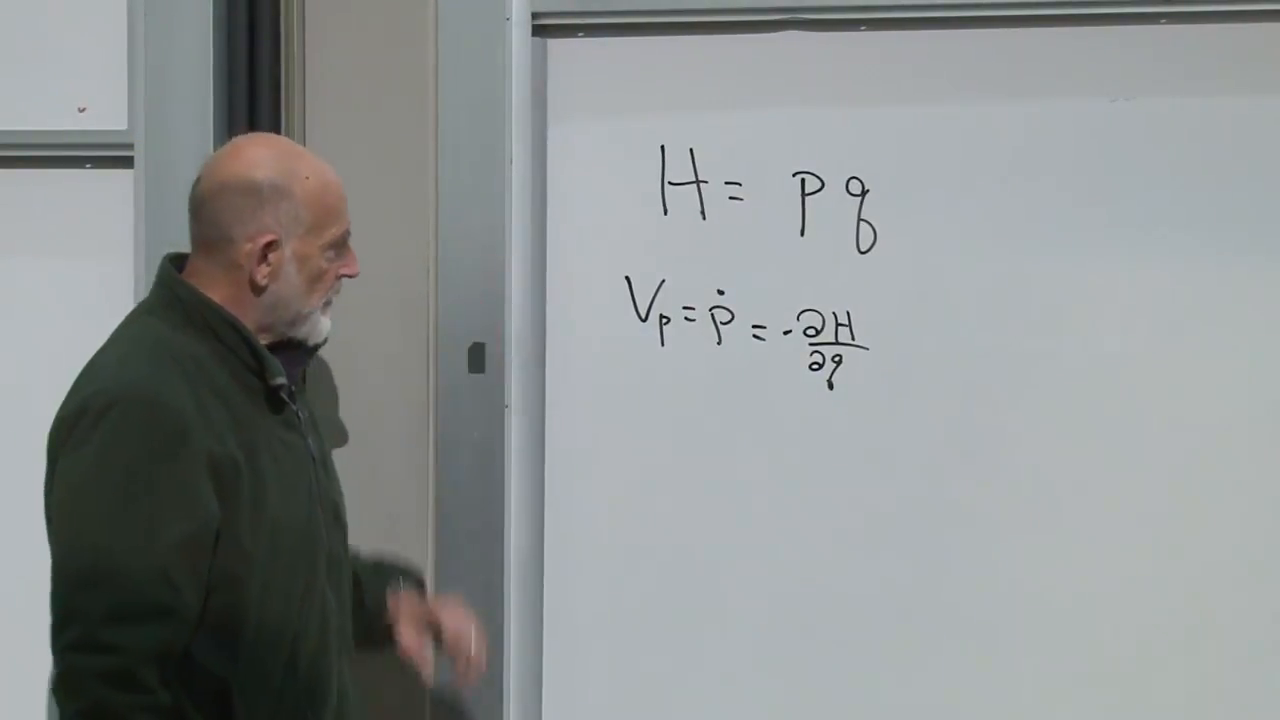
\includegraphics[width=0.82\textwidth]{lecture_07_figure_03.png}
  \caption{Phần mở đầu của ví dụ \(H=pq\) và thành phần vận tốc không gian pha
  đầu tiên.}
  \lectureframe{01:00:11}
\end{figure}

Các phương trình Hamilton là
\begin{equation}
  \dot p=-\lambda p,
  \qquad
  \dot q=\lambda q,
  \label{eq:l7-pq-flow}
\end{equation}
với nghiệm
\begin{equation}
  p(t)=p_0e^{-\lambda t},
  \qquad
  q(t)=q_0e^{\lambda t}.
  \label{eq:l7-pq-solutions}
\end{equation}
Một mảnh vuông bị ép co theo hàm mũ trong \(p\) và bị kéo giãn theo cùng hệ số
trong \(q\):
\begin{equation}
  \Delta p(t)\Delta q(t)
  =
  \Delta p(0)\Delta q(0).
  \label{eq:l7-pq-area}
\end{equation}
Độ phân kỳ của nó kiểm chứng kết quả này một cách cục bộ,
\begin{equation}
  \frac{\partial\dot p}{\partial p}
  +\frac{\partial\dot q}{\partial q}
  =-\lambda+\lambda=0.
  \label{eq:l7-pq-divergence}
\end{equation}

\begin{figure}[htbp]
  \centering
  \includegraphics[width=0.86\textwidth]{lecture_07_figure_11.png}
  \caption{Một mảnh gọn bị kéo dãn thành một dải dài mảnh trong khi vẫn bảo toàn
  diện tích dưới dòng \(H=pq\).}
  \lectureframe{01:02:10}
\end{figure}

\begin{classroomqa}
  \audiencequestion{Vì \(pq\) có đơn vị của tác dụng, định lý Liouville có phải là
  định luật bảo toàn tác dụng không? \lecturetimestamp{01:03:00--01:04:09}}
  \lecturerresponse{Không. Định lý này bảo toàn thể tích không gian pha. Trong một
  cặp chính tắc, \(dq\,dp\) có đơn vị của tác dụng, và sự kiện về thứ nguyên đó
  báo trước cơ học lượng tử, nơi các ô không gian pha được đo bằng các đơn vị
  do \(\hbar\) ấn định. Nhưng tích \(pq\) tự nó không phải là phiếm hàm tác dụng của Hamilton,
  cũng không tự động là mômen động lượng chỉ vì thứ nguyên trùng nhau.}
\end{classroomqa}

Ví dụ này cũng cho thấy các góc không nhất thiết được bảo toàn. Một hình chữ thập vuông góc
với các thành phần không bằng nhau, dưới phép co giãn trong
Phương trình ~\eqref{eq:l7-pq-solutions}, bị biến xén xét theo metric, trong khi diện tích
vẫn không đổi. Định lý Liouville là một định lý về diện tích hay thể tích,
không phải một định lý thông thường về tính cứng Euclid.

\section{Sự tắt dần tạo ra một điểm hút}

Để thấy định lý loại trừ điều gì, hãy xét phương trình rút gọn của một dao động tử tắt dần,
\begin{equation}
  m\ddot x=-kx-c\dot x,
  \qquad c>0.
  \label{eq:l7-damped-newton}
\end{equation}
Đặt \(p=m\dot x\). Khi đó
\begin{equation}
  \dot x=\frac{p}{m},
  \qquad
  \dot p=-kx-\frac{c}{m}p.
  \label{eq:l7-damped-first-order}
\end{equation}
Không có tắt dần, điểm pha quay quanh gốc tọa độ. Có tắt dần, năng lượng được truyền vào
các bậc tự do vi mô của môi trường xung quanh, và quỹ đạo xoắn ốc vào trong.

\begin{figure}[htbp]
  \centering
  \includegraphics[width=0.84\textwidth]{lecture_07_figure_13.png}
  \caption{Phương trình dao động tử tắt dần và đường xoắn ốc đi vào trong của nó trong
  mặt phẳng \(x\)-\(p\).}
  \lectureframe{01:13:30}
\end{figure}

Độ phân kỳ của dòng hai chiều rút gọn này là
\begin{equation}
  \frac{\partial\dot x}{\partial x}
  +\frac{\partial\dot p}{\partial p}
  =
  0-\frac{c}{m}<0.
  \label{eq:l7-damped-divergence}
\end{equation}
Mọi mảnh hữu hạn đều co lại. Gốc tọa độ là một điểm hút, tương tự liên tục
của sơ đồ trạng thái nhiều mũi tên đi vào.

\begin{figure}[htbp]
  \centering
  \includegraphics[width=0.88\textwidth]{lecture_07_figure_14.png}
  \caption{Các thành phần vận tốc không gian pha của hệ tắt dần dùng để thu được
  độ phân kỳ âm \(-c/m\).}
  \lectureframe{01:16:05}
\end{figure}

Điều này không có nghĩa là cơ học vi mô vi phạm định lý Liouville.
Hai biến \(x,p\) bỏ qua số lượng khổng lồ các bậc tự do của môi trường nhận năng lượng
của dao động tử. Hệ mở rộng gồm dao động tử cộng môi trường có thể là Hamilton và bảo toàn
thể tích dù mô tả rút gọn theo \(x,p\) của nó co lại.

\begin{classroomqa}
  \audiencequestion{Dao động tử tắt dần có còn được mô tả bởi phương trình Newton không, mặc dù nó không Hamilton trong không gian pha rút gọn này?
  \lecturetimestamp{01:20:09--01:21:12}}
  \lecturerresponse{Có. Phương trình \(F=ma\) của Newton có thể bao gồm một lực cản được đưa vào theo kinh nghiệm. Mô tả Lagrange sơ cấp \(L=T-V\) và mô tả Hamilton áp dụng trực tiếp cho các lực bảo toàn, và các Lagrangian tổng quát hơn cũng xử lý được một số lực phụ thuộc vận tốc. Tuy nhiên, một hạng ma sát Markov cho một cặp cô lập \(x,p\) là động lực học tiêu tán rút gọn, chứ không phải một hệ Hamilton chính tắc kín.}
\end{classroomqa}

\begin{classroomqa}
  \audiencequestion{Nếu các phương trình tắt dần có thể được tích phân ngược với độ chính xác vô hạn, thì thông tin có thật sự bị mất không?
  \lecturetimestamp{01:25:16--01:27:17}}
  \lecturerresponse{Với mọi thời gian hữu hạn, phương trình vi phân lý tưởng vẫn có nghịch đảo, nên dữ liệu chính xác có thể được chạy ngược lại. Phát biểu chính xác là các ô không gian pha hữu hạn co lại theo hàm mũ. Khi đó, việc khôi phục quá khứ của chúng đòi hỏi độ chính xác tăng theo hàm mũ, và ở thời gian vô hạn mọi quỹ đạo đều tiến tới điểm hút. Đây là phép tương tự cổ điển liên tục gần nhất với bức tranh rời rạc về sự mất các khả năng lựa chọn, chứ không phải khẳng định rằng hai nghiệm chính xác ở thời gian hữu hạn theo nghĩa đen trở thành một.}
\end{classroomqa}

\begin{classroomqa}
  \audiencequestion{Một trường vectơ có thể có phân kỳ bằng không mà không xuất phát từ một Hamiltonian không? \lecturetimestamp{01:18:21--01:22:34}}
  \lecturerresponse{Hoàn toàn có thể. Dạng Hamilton là điều kiện đủ cho phân kỳ bằng không, chứ không phải điều kiện cần. Một trường vận tốc không nén được bất kỳ có thể có phân kỳ bằng không mà không phải là một trường Hamilton chính tắc trên chính không gian ấy. Trường vận tốc của một chất lưu không nén được trong ba chiều là ví dụ điển hình trong lớp học: ba tọa độ tự chúng không thể tạo thành các cặp chính tắc. Cơ học chất lưu đầy đủ có thể có những mô tả Hamilton vô hạn chiều tinh vi hơn, nhưng điều đó không đảo ngược hàm ý một chiều đang được nêu ở đây.}
\end{classroomqa}

\section{Những phân biệt bổ sung được làm rõ qua các câu hỏi}

\begin{classroomqa}
  \audiencequestion{Chuyển động trên một mặt năng lượng không đổi liên hệ thế nào với sự bảo toàn toàn bộ một thể tích không gian pha?
  \lecturetimestamp{01:28:47--01:30:41}}
  \lecturerresponse{Đó là hai hệ quả độc lập của cấu trúc Hamilton. Nếu \(H\) không phụ thuộc thời gian, mỗi quỹ đạo sẽ ở lại trên mặt năng lượng riêng của nó. Một miền hữu hạn có thể cắt qua nhiều mặt như vậy; định lý Liouville nói rằng thể tích của toàn bộ miền ấy được bảo toàn. Đối với dao động tử điều hòa, miền ấy còn giữ nguyên hình dạng vì dòng là một phép quay cứng. Trong trường hợp \(H=pq\), miền ấy chỉ giữ diện tích chứ không giữ hình dạng.}
\end{classroomqa}

\begin{classroomqa}
  \audiencequestion{Công cơ học nằm ở đâu trong mô tả Hamilton? \lecturetimestamp{01:30:44--01:32:57}}
  \lecturerresponse{Công mô tả năng lượng được truyền qua một biên hệ được chọn. Một tác nhân bên ngoài có thể nâng một vật nặng hoặc thay đổi một tham số và do đó làm thay đổi năng lượng của hệ con; năng lượng nó cung cấp sẽ bị tác nhân mất đi. Nếu gộp cả hai phía vào trong một mô hình kín duy nhất, trọng tâm sẽ trở lại sự bảo toàn năng lượng toàn phần và sự trao đổi giữa các hệ con.}
\end{classroomqa}

\begin{classroomqa}
  \audiencequestion{Sự bảo toàn thể tích có đồng thời bảo toàn tôpô và các góc không? \lecturetimestamp{01:33:00--01:33:37}}
  \lecturerresponse{Một phép chảy Hamilton trơn trong thời gian hữu hạn bảo toàn tôpô vì nó là một phép biến dạng liên tục khả nghịch. Nói chung, nó không bảo toàn các góc Euclid hay hình dạng. Phép quay cứng của dao động tử thì có, nhưng sự kéo dãn \(H=pq\) cho thấy vì sao đó là một trường hợp đặc biệt.}
\end{classroomqa}

\begin{classroomqa}
  \audiencequestion{Việc bỏ qua phép biến đổi Legendre có phải vì nó không có ý nghĩa vật lý không? \lecturetimestamp{01:33:43--01:34:48}}
  \lecturerresponse{Không. Đó là phép biến đổi hữu ích hoán đổi mô tả theo vận tốc lấy mô tả theo xung lượng và tạo ra \(H=\sum_i p_i\dot q_i-L\) khi ánh xạ là chính quy. Phép dựng này đã được dùng lặp đi lặp lại ngay cả khi tên gọi hình thức của nó không được nhấn mạnh; đơn giản là lý thuyết tổng quát chi tiết chưa cần cho định lý hiện tại.}
\end{classroomqa}

\section{Ngoặc Poisson: bước nén tiếp theo}

Những phút cuối quay trở lại chủ đề lịch sử. Cơ học thế kỷ XIX đã nhiều lần tìm kiếm các cấu trúc gọn ghẽ liên kết những hệ có vẻ khác nhau---cơ học và quang học hình học, hạt và tia, quỹ đạo cổ điển và các mô tả kiểu sóng. Ngoặc Poisson là một cấu trúc như thế nữa, và chúng trở nên đặc biệt quan trọng trong cơ học lượng tử.

Cho \(F(q,p)\) là một hàm bất kỳ trên không gian pha. Nó có thể là một tọa độ, một xung lượng, tích \(qp\), hoặc mômen động lượng. Dọc theo chuyển động,
\begin{equation}
  \frac{dF}{dt}
  =
  \sum_i\left(
    \frac{\partial F}{\partial q_i}\dot q_i
    +\frac{\partial F}{\partial p_i}\dot p_i
  \right).
  \label{eq:l7-f-time-derivative}
\end{equation}
Thế các phương trình Hamilton vào:
\begin{equation}
  \frac{dF}{dt}
  =
  \sum_i\left(
    \frac{\partial F}{\partial q_i}
    \frac{\partial H}{\partial p_i}
    -
    \frac{\partial F}{\partial p_i}
    \frac{\partial H}{\partial q_i}
  \right).
  \label{eq:l7-f-hamiltonian-derivative}
\end{equation}

\begin{figure}[htbp]
  \centering
  \includegraphics[width=0.88\textwidth]{lecture_07_figure_15.png}
  \caption{Quy tắc chuỗi cho đạo hàm theo thời gian của một hàm không gian pha tổng quát \(F(q,p)\).}
  \lectureframe{01:42:40}
\end{figure}

Tổ hợp phản đối xứng lặp đi lặp lại này xứng đáng có một tên gọi. Với hai hàm bất kỳ \(F\) và \(G\), định nghĩa ngoặc Poisson của chúng bởi
\begin{equation}
  \boxed{
  \{F,G\}
  =
  \sum_i\left(
    \frac{\partial F}{\partial q_i}
    \frac{\partial G}{\partial p_i}
    -
    \frac{\partial F}{\partial p_i}
    \frac{\partial G}{\partial q_i}
  \right).}
  \label{eq:l7-poisson-bracket}
\end{equation}

\begin{figure}[htbp]
  \centering
  \includegraphics[width=0.86\textwidth]{lecture_07_figure_16.png}
  \caption{Tổ hợp đạo hàm của hai hàm khi được nâng thành ngoặc Poisson.}
  \lectureframe{01:44:15}
\end{figure}

Phương trình~\eqref{eq:l7-f-hamiltonian-derivative} trở thành
\begin{equation}
  \boxed{\frac{dF}{dt}=\{F,H\}.}
  \label{eq:l7-hamiltonian-poisson-evolution}
\end{equation}
Nếu \(F\) còn phụ thuộc tường minh vào thời gian, ta thêm \(\partial F/\partial t\). Lấy \(F=q_i\) hoặc \(F=p_i\) thì thu lại được hai phương trình Hamilton, vì vậy phương trình~\eqref{eq:l7-hamiltonian-poisson-evolution} là một dạng cô đọng của toàn bộ động lực học.

Ký hiệu luôn có thể bị nén một cách nhân tạo---người ta có thể bình phương nhiều phương trình, cộng chúng lại, rồi gọi kết quả là một phương trình. Làm như vậy sẽ che giấu chứ không làm lộ ra cấu trúc. Ngoặc Poisson hữu ích vì lý do ngược lại: đại số của nó tổ chức sự tiến hóa theo thời gian, các đại lượng bảo toàn và đối xứng. Bước tiếp theo là phát triển đại số ấy rồi dùng nó cho mômen động lượng, mà cấu trúc của nó sẽ giữ vai trò trung tâm cả trong cơ học cổ điển lẫn trong lý thuyết lượng tử.

\section{Ý nghĩa liên tục của tính thuận nghịch}

Giờ đây ta có thể phát biểu chuỗi ý tưởng ấy mà không rút ngắn nó. Các phương trình Hamilton bảo toàn \(H\) khi Hamiltonian không phụ thuộc tường minh vào thời gian, nên các quỹ đạo riêng lẻ nằm trên các siêu mặt năng lượng không đổi. Cũng chính các phương trình ấy gán một vận tốc cho mỗi điểm của không gian pha. Phân kỳ của vận tốc đó triệt tiêu vì các đạo hàm riêng hỗn hợp khử nhau từng cặp. Do đó, toàn bộ một miền các trạng thái khả dĩ bảo toàn thể tích chính tắc của nó.

Đó là phiên bản liên tục của một mũi tên đi vào và một mũi tên đi ra. Hình dạng có thể thay đổi, các góc có thể thay đổi, và các quỹ đạo lân cận có thể tách xa nhau rất nhiều. Điều không thể xảy ra trong một mô tả Hamilton kín, trơn là việc nén một tập hữu hạn các khả năng lựa chọn vào một thể tích không gian pha nhỏ hơn. Dòng \(H=pq\) cho thấy sự tự do kéo dãn; dao động tử tắt dần rút gọn cho thấy điểm hút xuất hiện khi các điều kiện Hamilton bị từ bỏ. Khi đó, ngoặc Poisson cô đọng cùng một động lực học vào mệnh đề rằng Hamiltonian sinh ra mọi đạo hàm theo thời gian.
